
\de{ĐỀ THI GIỮA HỌC KỲ II NĂM HỌC 2022-2023}{THPT Nguyễn Du}

\begin{bt}%[Dự án đề kiểm tra GHKII NH22-23- Hiếu Mai]%[0T7Y1-1]%Câu 1
	Tìm tất cả các giá trị thực của tham số $m$ để $f(x)=(m^2-4)x^2-2mx-m-3$ là một tam thức bậc hai.
	\loigiai{
Ta có $f(x)$ là tam thức bậc hai khi $m^2-4 \ne 0  \Leftrightarrow \heva {&m\ne 2 \\& m \ne -2.}$
	}
\end{bt}

\begin{bt}%[Dự án đề kiểm tra GHKII NH22-23- Hiếu Mai]%[0T8Y1-2]%Câu 2
	Bình đến văn phòng phẩm mua quà tặng bạn, trong cửa hàng có $12$ quyển vở khác nhau, $5$ loại bút khác nhau. Hỏi Bình có bao nhiêu cách chọn quà gồm $1$ quyển vở và $1$ cây bút?
	\loigiai{
	Theo quy tắc nhân, số cách chọn phần quà gồm một quyển vở và một cây bút là\\
	$12 \cdot 5 =60$ cách.
	}
\end{bt}

\begin{bt}%[Dự án đề kiểm tra GHKII NH22-23- Hiếu Mai]%[0T7B2-1]%Câu 3
	Giải bất phương trình $(2x-1)^2\leq x+10$.
	\loigiai{ Ta có 
		\allowdisplaybreaks \vspace*{-0.7cm}
	\begin{eqnarray*} 
		&  & (2x-1)^2\leq x+10 \\
		&  \Leftrightarrow  & 4x^2 -4x+1 -x -10\leq 0\\ 
		&  \Leftrightarrow  & 4x^2 -5x -9 \leq 0
	\end{eqnarray*}
	Dựa vào bảng xét dấu
	\begin{center}
			
\begin{tikzpicture}[font=\normalsize,t style/.style={style=solid}]
				\tkzTabInit[nocadre=false,lgt=3.5,espcl=1.5,deltacl=0.5]
				{$x$ /1, $4x^2 -5x -9$/0.75}
				{$ -\infty $,$ -1 $,$ \dfrac{9}{4} $,$ +\infty $}
				\tkzTabLine{  , +,0 , -,0  , +,  }  
			\end{tikzpicture}
		\end{center}
ta thấy tập nghiệm của bất phương trình là $S=\left[-1;\dfrac{9}{4}\right]$.
	}
\end{bt}

\begin{bt}%[Dự án đề kiểm tra GHKII NH22-23- Hiếu Mai]%[0T7B3-2]%Câu 4
	Giải phương trình $\sqrt{x^2-3x+1}=x-1$.
	\loigiai{
Ta có	\allowdisplaybreaks \vspace*{-0.7cm}
\begin{eqnarray*} 
	&  & \sqrt{x^2-3x+1}=x-1 \\
	&   \Rightarrow   & x^2 -3x+1 = (x-1)^2\\ 
	&  \Rightarrow  & x^2 -3x +1 =x^2 -2x+1\\
	&  \Rightarrow  & x=0
\end{eqnarray*}	
Thử $x=0$ vào phương trình ta thấy không thỏa mãn.\\
Vậy bất phương trình đã cho vô nghiệm. Tập nghiệm $S=\varnothing$. 
}
\end{bt}

\begin{bt}%[Dự án đề kiểm tra GHKII NH22-23- Hiếu Mai]%[0T7B1-1]%Câu 5
	Cho tam thức bậc hai $f(x)=-x^2+2(m+1)x-4$. Tìm tham số $m$ để $f(x)<0$ với mọi $x \in \mathbb{R}$.
	\loigiai{
	Tam thức bậc hai $f(x)=-x^2+2(m+1)x-4$ có $a=-1$, $b'=m+1$, $c=-4$.\\
	$\Delta'= (m+1)^2-(-1)\cdot (-4)=m^2+2m-3$.\\
	Ta có
	\allowdisplaybreaks
	$\begin{aligned}[t]
	f(x)<0,\, \forall x \in \mathbb{R}
		  \Leftrightarrow & \heva{&a<0\\&\Delta'<0}\\
		  \Leftrightarrow & \heva{&-1<0\\ & m^2+2m-3<0}\\
		   \Leftrightarrow & -3<m<1.
	\end{aligned}$\\
Vậy $-3<m<1$ thỏa đề bài.
	}
\end{bt}

\begin{bt}%[Dự án đề kiểm tra GHKII NH22-23- Hiếu Mai]%[0T8B1-3]%Câu 6
	Mỗi đội bóng có $6$ cầu thủ ra sân. Trước một trận thi đấu bóng đá tại sân trường Nguyễn Du, mỗi cầu thủ của đội này bắt tay với $6$ cầu thủ của đội kia	và $3$ trọng tài. Tính tổng số cái bắt tay.
	\loigiai{
	$\bullet$ Số cái bắt tay giữa các cầu thủ của hai đội là $6\cdot 6=36$ cái.\\
	$\bullet$ Số cái bắt tay giữa các cầu thủ hai đội với $3$ trọng tài là $12\cdot 3 =36$ cái.\\
	Tổng số cái bắt tay của trận đấu là $36+36=72$ cái.
	}
\end{bt}

\begin{bt}%[Dự án đề kiểm tra GHKII NH22-23- Hiếu Mai]%[0T9B1-5]%Câu 7
	Trong mặt phẳng $Oxy$, cho ba điểm $A(m;4)$, $B(2;-4)$, $C(6;0)$.
	Định tham số $m$ để ba điểm $A, B, C$ thẳng hàng.
	\loigiai{
	Ta có $\vec{BA}=(m-2;8)$; $\vec{BC}=(4;4)$.\\
	Ba điểm $A,B,C$ thẳng hàng khi $\vec{BA}$ và $\vec{BC}$ cùng phương\\
	$ \Leftrightarrow 4(m-2)=8\cdot 4  \Leftrightarrow m=10$.\\
	Vậy $m=10$ thỏa đề bài. 
	}
\end{bt}

\begin{bt}%[Dự án đề kiểm tra GHKII NH22-23- Hiếu Mai]%[0T9B2-2]%Câu 8
	Trong mặt phẳng $Oxy$, cho tam giác $ABC$ biết $A(-1;-2)$, $B(0;4)$, $C(2;2)$. Viết phương trình đường cao $BH$ của tam giác $ABC$.
	\loigiai{
	$\bullet$ Vì $BH \perp AC$ nên $BH$ có véc-tơ pháp tuyến là $\vec{n}= \vec{AC}=(3;4)$.\\
	$\bullet$ Mà $BH$ qua $B(0;4)$ nên $BH$ có phương trình là
$$3(x-0)+4(y-4)=0 \Leftrightarrow 3x+4y-16=0.$$
	}
\end{bt}

\begin{bt}%[Dự án đề kiểm tra GHKII NH22-23- Hiếu Mai]%[0T9K3-3]%Câu 9
\immini [thm]{Trong mặt phẳng $Oxy$, một vật chuyển động tròn đều ngược chiều kim đồng hồ trên đường tròn tâm	$I(2;2)$ bán kính $R=5$. Dưới tác dụng của lực căng tác dụng lên sợi dây $IM$. Khi vật chuyển động tới điểm $M(5; 6)$ thì dây căng bị đứt (tham khảo hình vẽ). Viết phương trình quỹ đạo $Mt$ chuyển động của vật sau khi dây bị đứt (biết vật chỉ chịu tác động duy nhất lực căng dây).
}
{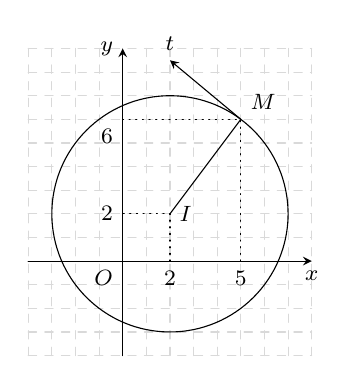
\begin{tikzpicture}[scale=0.3,>=stealth, font=\footnotesize, line join=round, line cap=round]
		\def\a{1} \def\b{-4} \def\c{3} % Hệ số
		\def\xmin{-4} \def\xmax{8}
		\def\ymin{-4} \def\ymax{9}
		\draw[color=gray!30,dashed] (\xmin,\ymin) grid (\xmax,\ymax);	
		\draw[->] (\xmin,0)--(\xmax,0) node [below]{$x$};
		\draw[->] (0,\ymin)--(0,\ymax) node [left]{$y$};
		\node at (0,0) [below left]{$O$};
%		\clip (\xmin+0.1,\ymin+0.1) rectangle (\xmax-0.1,\ymax-0.1);
		\draw (2,2) circle (5 cm) node[right] {$I$} (2,2)--(5,6);
		\draw[->] (5,6) node [above right]{$M$}--++(-3,2.5) node [above]{$t$};
		\draw[dotted] (5,0) node[below] {$5$}|-(0,6)node[below left] {$6$}  (2,0)node[below] {$2$}|-(0,2)node[left] {$2$};
	\end{tikzpicture}
}
	\loigiai{
Ta có $\vec{IM}=(3;4)$.\\
Theo đề bài, quỹ đạo chuyển động của vật là tia $Mt$ nằm trên tiếp tuyến tại $M$ của đường tròn (theo phương có hoành độ âm).\\
Tia $Mt$ có một véc-tơ chỉ phương là $\vec{u}=(-4;3)$.\\
Phương trình quỹ đạo $Mt$ là $\heva{&x=5-4t\\&y=6+3t}$ với $t>0$.	
	}
\end{bt}

\begin{bt}%[Dự án đề kiểm tra GHKII NH22-23- Hiếu Mai]%[0T9K2-6]%Câu 10
	Trong mặt phẳng $Oxy$, cho đường thẳng $d\colon \heva{&x=1-t\\&y=1+2t}$ và
	điểm $M(-5;3)$. Tìm tọa độ hình chiếu vuông góc của điểm $M$ trên đường thẳng $d$.
	\loigiai{
	$\bullet$ Đường thẳng $d$ có véc-tơ chỉ phương là $\vec{u}=(-1;2)$.\\
	$\bullet$ Gọi $H(1-t;1+2t)\in d$ là hình chiếu của $M(-5;3)$ lên đường thẳng $d$.\\
	Khi đó $\vec{MH}=(6-t;-2+2t)$.\\
	$\bullet$ $\vec{u} \perp \vec{MH}  \Leftrightarrow -1(6-t)+2(-2+2t)=0 \Leftrightarrow 5t-10=0 \Leftrightarrow t=2$.\\
	Vậy hình chiếu của $M$ lên $d$ là $H(-1;5)$.
}
\end{bt}


